\documentclass{article}

% supress page numbering so that a single eps figure can be generated:
\usepackage{nopageno}

\usepackage{tikz}
\usetikzlibrary{bayesnet}

\begin{document}

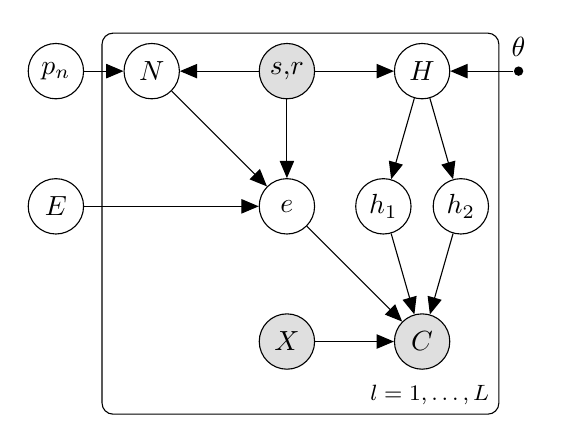
\begin{tikzpicture}
  \node[obs] (C) {$C$} ;
  \node[obs, left=of C] (X) {$X$} ;
  \node[latent, above=of X] (e) {$e$} ;
  \node[obs, above=of e] (sr) {$s$,$r$} ;
  \node[latent, left=of sr] (N) {$N$} ;
  \node[latent, left=0.5 of N] (pn) {$p_n$} ;
  \node[latent, below=of pn] (E) {$E$} ;
  \node[latent, right=of sr] (H) {$H$} ;
  \node[latent, below=of H, xshift=-14] (h1) {$h_1$} ;
  \node[latent, below=of H, xshift= 14] (h2) {$h_2$} ;
  \node[left=-0.1 of N] (plateSpace) {};
  \node[circle,fill,inner sep=1.2pt, right=0.8 of H, label=above:\fontsize{10}{10}\selectfont$\theta$] (theta) {};
  \edge {E,N,sr} {e} ;
  \edge {X,e,h1,h2} {C} ;
  \edge {pn,sr} {N} ;
  \edge {H} {h1,h2} ;
  \edge {sr,theta} {H}
  \plate {lplate} {(N)(sr)(e)(H)(h1)(h2)(X)(C)(plateSpace)} {$l = 1,\ldots,L$}
\end{tikzpicture}

\end{document}
